A parallel Monte Carlo simulation was written to model surface plasmon
polariton multiple scattering.
It assumes the geometry shown in \Figure{fig:plasmongeo} consisting of
\begin{itemize}
  \item An elliptical \textit{illuminated region}, representing the incident evanescent
        field used to excite plasmons on the surface.  This ellipse has
        typical radii $r_a=\SI{5}{\micro\meter}$ and $r_b=\SI{3}{\micro\meter}$.
  \item A \textit{tip}, a single movable scatterer.
  \item The \textit{scan area}, a square area wherein the tip rasters, typically
        $128\times128$ points in a maximal area of $2.27\times\SI{2.27}{\micro\meter}$.
  \item \textit{Scatterers}, fixed point scatterers (usually \num{20})
        distributed randomly in a square of $8.8281\times\SI{8.8281}{\micro\meter}$
        where the plasmon can visit, and
  \item A \textit{trajectory} or \textit{path} meaning the ordered sequence of scatterers a
        plasmon visits before exiting the system.  The trajectory has a typical maximum
        path length of \SI{18}{\micro\meter}.
\end{itemize}
\begin{figure}[ht]
  \centering
  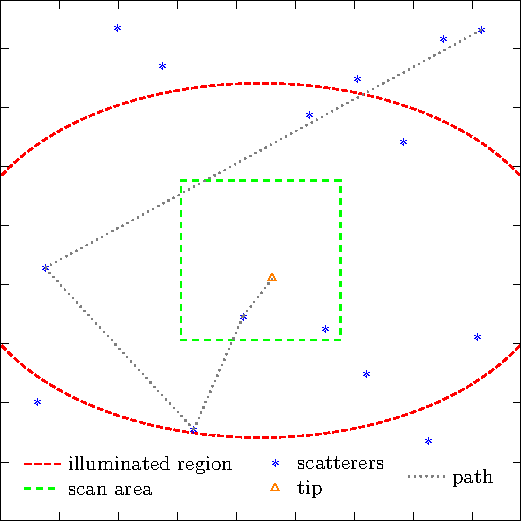
\includegraphics[keepaspectratio]{scatteringmicro/figures/montecarlogeo.pdf}
  \caption{Definition of terms: geometry for the Monte Carlo scattering
    simulation}
  \label{fig:plasmongeo}
\end{figure}

The plasmon is assumed to be a time independent monochromatic plane wave
of the form $E(\mathbf{r})=\me^{\mi \ksp\mathbf{r}}$, where
$\ksp$ is the plasmon wavevector and $\mathbf{r}$ is some
spatial variable.  The plasmon trajectories are modeled as follows:
First, a random scatterer with index $n$ and coordinates $(x_n,y_n)$ is
chosen within the illuminated region as the first scatterer a plasmon
visits.  Since the illuminated region always encloses the scan area, we are
guaranteed at least one scatterer (the tip) to choose from.  The plasmon
initializes with local phase $\varphi_\mathrm{l,n}=\ksp x_n$
representing the local phase advance from the (arbitrary) point where the
plasmon is excited by the (linear in either $x$ or $y$) evanescent field to
the first scatterer.  Next, scatterers are randomly and sequentially chosen
from amongst all possible scatterers including the tip and the total path
length accumulated as the plasmon visits each scatterer.  The trajectory
ends when
\begin{itemize}
  \item The same scatterer is visited twice in a row, or
  \item The total accumulated path length exceeds a pre-defined limit based
        on the \gls{spp} $1/\me$ propagation length.
\end{itemize}
This process is repeated many times for each tip position in the scan area.
Usually \numrange{250000}{1000000} trajectories will be used for each point
of the $128\times128$ grid.  During this process the path length, and
therefore the total phase from multiple scattering at $K$ sites
\begin{align}
  \varphi_\mathrm{ms,n}=\sum_{k=0}^{K-1}\sqrt{{(x_{k+1}-x_k)}^2+{(y_{k+1}-y_k)}^2}
\end{align}
is, along with the final scatterer, saved.

The ultimate output from the Monte Carlo simulation consists of {\it
    topology maps}, colloquially dubbed \textit{weirdospace}, having the same pixel
dimensions as the scan area.  Each weirdospace image represents, for each
pixel, the far field phase and intensity of a particular point at a certain
angle along the plasmon ring for the respective tip position in the scan
area.  The weirdospace image for each angle $\phi$ along the ring is
calculated by adding a final phase $\varphi_\mathrm{ff,n}$ equal to the
propagation from the final scatterer to the far field along plasmon
scattering angle $\theta_\mathrm{sp}$.  This is
\begin{align}
  \varphi_\mathrm{ff,n} = k_0 \sin
  \theta_\mathrm{sp}\left(x_n\cos\phi+y_n\sin\phi\right)
\end{align}
Where $\ksp=k_0\sin \theta_\mathrm{sp}$.  Each path therefore
represents a wave of the form
\begin{align}
  E_n=\me^{\mi(\varphi_\mathrm{l}+\varphi_\mathrm{ms}+\varphi_\mathrm{ff})}
\end{align}
And the total far field intensity is the linear superposition of these
waves
\begin{align}
  E_\mathrm{total}(\phi) =
  \left|\sum_{n=0}^{N} E_n\right|^2
\end{align}

In total, the program writes the following data
\begin{itemize}
  \item Weirdospace images in a 64 bit floating point HDF5 files.  The images
        are names {\tt XXXXX-scatter.h5}, where {\tt XXXXX} represents the angle
        in degrees of that particular frame along the ring.  Both the phase and
        intensity are stored in each file.
  \item {\tt ring.dat}, a tab separated values file containing the angle,
        mean intensity, and variance of intensity for each weirdospace image.  This
        file is no longer created by the main program, but computed from the output
        by a supporting script {\tt mkring.sh}.
  \item {\tt parameters}, a file containing program variables, scatterer
        locations, and statistics.  The parameters are as shown in \Table{tbl:parameters}.
        \begin{table}
          \begin{center}
            \begin{tabular}{ll}
              \toprule
              parameter          & description                                     \\
              \midrule
              {\tt SX}, {\tt SY} & integer size of scan area                       \\
              {\tt ELLIPSE\_A}   & first radius of elliptical illuminated area     \\
              {\tt ELLIPSE\_B}   & second radius of elliptical illuminated area    \\
              {\tt LAMBDA}       & wavelength of incident light, in microns        \\
              {\tt PATHLEN}      & maximum path length for a plasmon               \\
              {\tt ENTIREAREA}   & square boundary for random scatterer generation \\
              {\tt SCANAREA}     & dimensions of the scan area in microns          \\
              {\tt EVENTS}       & events per point in the scan area               \\
              {\tt NSCAT}        & number of randomly distributed scatterers       \\
              \bottomrule
            \end{tabular}
          \end{center}
          \caption{Explanation of variables used in the {\tt parameters} file.}
          \label{tbl:parameters}
        \end{table}
        At the end there is a section called {\tt STATS}.  The first column of this
        section represents the number of scatterers visited, the second the
        percentage of all trajectories including exactly this many scatterers, and
        the third column the percentage of those trajectories included the tip in
        some way.  The first row is the sum of all the following data.
\end{itemize}

The weirdospace images are colored in such a way as to show both phase and
intensity information at the same time.  This is done by mapping the
information onto a circular coordinate system as shown in \Figure{fig:hsv}, where the intensity is mapped to the magnitude of the radial
component $r$ and phase to the angle $\theta$.
\begin{figure}[ht]
  \centering
  %\begin{center}
  %\psset{unit=1cm}
  %% made this picture with the gimp... has HSV effect built right in
  %\begin{overpic}[width=5.0cm,height=5.0cm]{simulation/hsvradial.eps}
  %\begin{pspicture}(-2.5,-2.5)(2.5,2.5)
  %\pnode(0,0){C} % center
  %\pnode(! 90 sin 2.5 mul 90 cos 2.5 mul){A} % edge 1
  %\pnode(! 55 sin 2.5 mul 55 cos 2.5 mul){B} % edge 2
  %\psset{linecolor=white}
  %\ncline{->}{C}{B}\taput{{\white$r$}} % line to edge 2
  %\ncline{->}{C}{A} % line to edge 1
  %\pstMarkAngle[]{A}{C}{B}{{\white$\theta$}} % mark the angle
  %\end{pspicture}
  %\end{overpic}
  %\end{center}
  \caption{Weirdospace images are colored by using the above model based on a
    circular coordinate system.  Intensity is mapped to the radial component
    $r$ and phase the angle $\theta$.}
  \label{fig:hsv}
\end{figure}
This coding scheme is identical to that which can be produced in HSV color
space with the saturation always being set to unity.

\subsubsection{Statistics}
\begin{figure}[ht]
  \centering
  \import{includes/}{setpgfinc}
  \import{scatteringmicro/figures/}{pdfpicking}
  %\begin{center}
  %\psset{xAxisLabel=,yAxisLabel=}
  %\begin{psgraph}(0,0)(1.5,1.5){10cm}{4cm}
  %\psplot[linecolor=red]{0}{1}{x dup mul 4 x mul sub PI add 2 x mul mul}
  %\psplot[linecolor=red]{1}{1.4142}{4 x dup mul 1 sub sqrt mul x dup mul 2
  %add PI sub sub 4 x dup mul 1 sub sqrt ATAN mul sub 2 x mul mul}
  %\psplot[linecolor=blue]{0}{1}{4 x mul PI 0.5 dup mul mul div x 2 0.5 mul
  %div ACOS mul 2 x dup mul mul PI 0.125 mul div 1 x dup mul sub 4 0.5 dup mul
  %mul div sqrt mul sub}
  %\psxTick(1.4142){\sqrt{2}} % max distance for a square
  %\end{psgraph}
  %\end{center}
  \caption{Probability distribution function for the square and disk line
    picking problems.}
  \label{fig:linepickingpdf}
\end{figure}
The way we choose scattering trajectories in the simulation leads to an
interesting statistical distribution for the number of scatterers visited.
Again, there are two criteria which can end a trajectory
\begin{itemize}
  \item The same scatter is chosen twice.
  \item The path length reaches a hard limit.
\end{itemize}
The first exit criteria was chosen ostensibly to provide for the strong
presence of single scattering off the tip.  Consider a rectangular area
containing $N$ scatterers.  The probability at each scatterer of choosing
pairwise sequential the same scatterer is $1/N$.  The extension of this to
the probability of the path ending on the $n$th scattering site, $P(n)$, is
modeled by the familiar differential equation for exponential decay
\begin{align}
  \frac{d P(n)}{dn} = -\frac{1}{N}P(n)
\end{align}
which, when solved and the initial condition $P(0)=1/N$ is applied, can be
expressed as
\begin{align}
  P(n)=\frac{1}{N}e^{-n/N}
\end{align}
%separation of variables results in
%\begin{align}
%\frac{d P(n)}{P(n)}=-\frac{1}{N}dn
%\end{align}
%integrating yields
%\begin{align}
%\log P(n) = -\frac{n}{N} + C
%\end{align}
%and therefore
%\begin{align}
%P(N)= e^C e^{-n/N}
%\end{align}
%The initial condition represented by $e^C$ is found by noting $P(0)=1/N$,
%therefore the final form of this equation is given by
This is the lifetime of the plasmon trajectory considering its only exit
possibility is due to choosing the same scatterer twice.

The second exit criteria comes when our path length has been exhausted.
Since the scatterers are randomly distributed throughout the area, it is
useful to know the mean free path for such a system.  Consider a unit
square.  The average distance between any two points is given by the box
integral
\begin{align}
  \int_0^1 \int_0^1 \int_0^1 \int_0^1 \sqrt{(x_1-y_1)+(x_2-y_2)}\; dx_1 dx_2 dy_1 dy_2
\end{align}
This is the \textit{square line picking} problem.  Analytic evaluation of the
above integral is complicated, but yields for its unit dimensions an
average distance of
\begin{align}
  \overline{r} = \frac{\sqrt{2}+2+5\log\left(1+\sqrt{2}\right)}{15}
\end{align}
and the probability distribution
\begin{align}
  P_\mathrm{s}(l) = \left\{
  \begin{array}{l l}
    2l\left(l^2 -4l + \pi\right) & \quad  0\leq l \leq 1        \\
    2l\left[4\sqrt{l^2-1}-\left(l^2+2-\pi\right)-4\arctan\left({\sqrt{l^2-1}}\right)\right]
                                 & \quad 0 \leq l \leq \sqrt{2} \\
  \end{array}
  \right.
\end{align}
If we instead suppose a unit disk instead of a unit square, the mean
distance can be found to be
\begin{align}
  \overline{r}= \frac{128}{45 \pi}
\end{align}
and probability distribution for a disk of radius $R$ is
\begin{align}
  P_\mathrm{d}(l)=\frac{4l}{\pi R^2} \arccos\left(\frac{l}{2R}\right) - \frac{2
    l^2}{\pi R^3} \sqrt{1-\frac{l^2}{4 R^2}}
\end{align}
It is assumed that the superposition of the two probabilities should
produce the statistical results found \Figure{fig:linepickingpdf}, but as yet
I have not found a way to do so.

These line picking problems are useful because they characterize how many
scatterers on average a plasmon will visit until exiting in the Monte Carlo
simulation.  They also reveal a limitation: as the scattering density is
increased, a plasmon as simulated does not visit more scatterers, nor does
its mean free path decrease.  Rather, the result of increasing the number
of scatterers is only to suppress single scattering off the tip.  This may
or may not be physical.
